%!TEX root = ../main.tex



\section{Εισαγωγή}

\lettrine[findent=2pt]{\fbox{\textbf{Σ}}}{ε} αυτό το κεφάλαιο θα παρουσιαστούν τα πειράματα που έγιναν έτσι ώστε να υπάρχει εφαρμογή στην πράξη της θεωρίας και όσων έχουν αναφερθεί στα προηγούμενα κεφάλαια. Με αυτόν τον τρόπο μελετάται και κατά πόσο ο ελεγκτής που σχεδιάστηκε είναι ικανός να ελέγξει ικανοποιητικά διάφορα συστήματα ελέγχου. Σε κάθε ενότητα θα παρουσιάζεται ένα από τα διαθέσιμα συστήματα, το μαθηματικό μοντέλο του και τα αποτελέσματα του ελέγχου που παρέχει ο αυτο-ρυθμιζόμενος PID ελεγκτής. Τέλος, η κάθε ενότητα κλείνει με το σχολιασμό των πειραματικών αποτελεσμάτων.

\section{Σύστημα Mass-Springer-Damper}

\subsection{Μαθηματικό Μοντέλο}

Το πρώτο σύστημα που θα αναλυθεί είναι το σύστημα Μάζα-Ελατήριο-Αποσβεστήρας (Σχήμα \ref{fig:mass_spring_damper}) που αποτελεί ένα από τα πιο κλασικά συστήματα ελέγχου καθώς οι δυναμικές σχέσεις που το διέπουν δεν είναι περίπλοκες και είναι εύκολη η κατανόηση τους.

\begin{figure}[h]
  \centering
  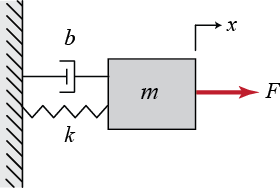
\includegraphics[width=\textwidth,height=5cm,keepaspectratio]{mass_spring_damper}
  \caption{Μοντέλο συστήματος Μάζας-Ελατηρίου-Αποσβεστήρα}
  \label{fig:mass_spring_damper}
\end{figure}

\noindent
H διαφορική εξίσωση που χαρακτηρίζει το σύστημα αυτό είναι
\begin{equation}
m\ddot{x} + b\dot{x} + kx = F
\label{eq:mass_springer_damper_ode}
\end{equation}
όπου $m$ είναι η μάζα, $x$ είναι η μετατόπιση της μάζας από το σημείο ισορροπίας, $b$ είναι η απόσβεση που παρέχει ο αποσβεστήρας, $k$ είναι η σταθερά του ελατηρίου και $F$ είναι η δύναμη που ασκείται στο σύστημα. Παίρνοντας το μετασχηματισμό Laplace της παραπάνω εξίσωσης έχουμε
\begin{equation}
ms^2X(s) + bsX(s) + kX(s) = F(s)
\label{eq:mass_springer_damper_laplace}
\end{equation}
Συνεπώς η συνάρτηση μεταφοράς (\emph{Transfer Function}) μεταξύ της εισόδου, που είναι η δύναμη $F(s)$, και της εξόδου, που είναι η μετατόπιση της μάζας $X(s)$, είναι
\begin{equation}
\frac{X(s)}{F(s)} = \frac{1}{ms^2 + bs + k}
\end{equation}

\subsection{Πείραμα}

Έστω ότι $\displaystyle m = 1\ kg$, $\displaystyle b = 10\ \frac{Ns}{m}$, $\displaystyle k = 20\ \frac{N}{m}$, $\displaystyle F = 1\ N$. Αντικαθιστώντας αυτές τις τιμές στην εξίσωση \ref{eq:mass_springer_damper_laplace} έχουμε
\begin{equation}
\frac{X(s)}{F(s)} = \frac{1}{s^2 + 10s + 20}
\end{equation}

\subsubsection{Απόκριση Χωρίς Έλεγχο}

Στο Σχήμα \ref{fig:mass_springer_damper_no_control} φαίνεται η βηματική απόκριση του συστήματος όταν δεν υπάρχει έλεγχος. Καθίσταται εμφανές ότι από μόνο του το σύστημα έχει μη ικανοποιητική απόκριση καθώς η τελική τιμή της εξόδου του είναι $y(t) = 0,047619$ και έχει ποσοστό σφάλματος \textit{offset error}$= 95.238 \%$. Συνεπώς κρίνεται απαραίτητη η χρήση ελεγκτή. Τα κέρδη του θα υπολογιστούν χρησιμοποιώντας τη μέθοδο αυτο-ρύθμισης που έχει περιγραφεί.

\begin{figure}[h]
  \centering
  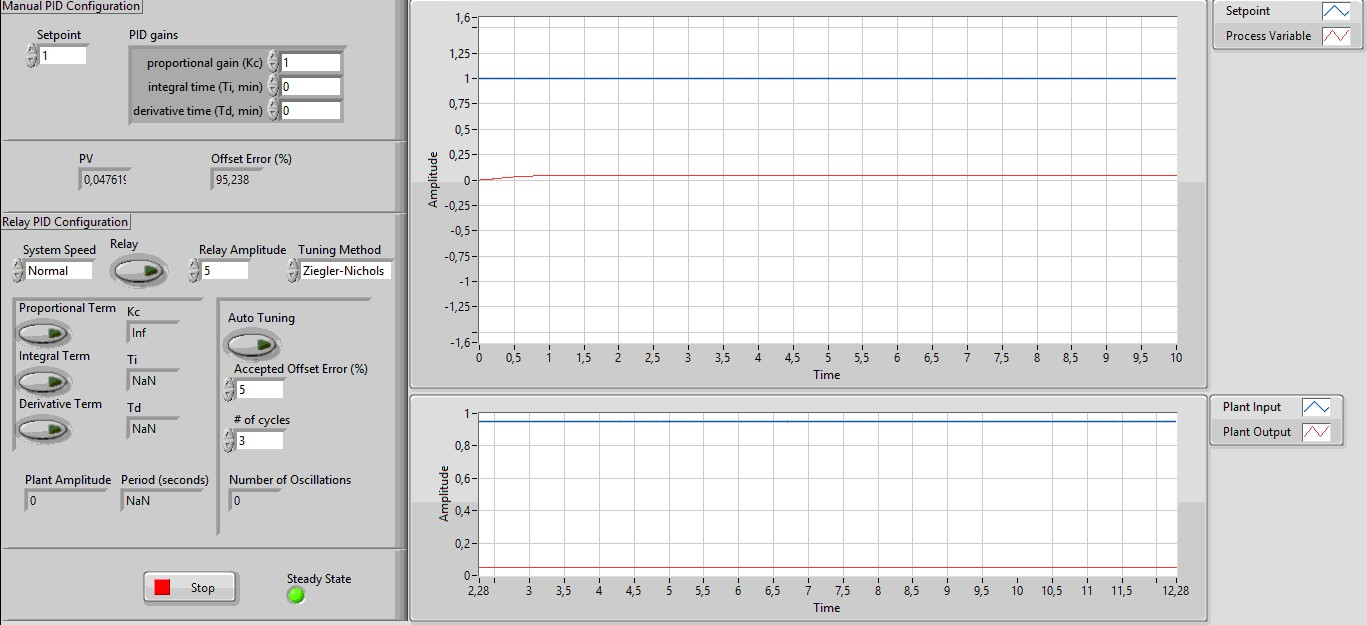
\includegraphics[width=\textwidth,height=5cm,keepaspectratio]{mass_springer_damper_no_control}
  \caption{Βηματική απόκριση του συστήματος Μάζα-Ελατήριο-Αποσβεστήρας χωρίς έλεγχο}
  \label{fig:mass_springer_damper_no_control}
\end{figure}

\subsubsection{Αναλογικός Έλεγχος}

Στο Σχήμα \ref{fig:mass_springer_damper_proportional_control} φαίνεται η βηματική απόκριση του συστήματος όταν σε αυτό εφαρμόζεται αναλογικός έλεγχος. Το κέρδος $K_c$ του αναλογικού όρου υπολογίστηκε αυτόματα, χρησιμοποιώντας τους τύπους από τη μέθοδο Ziegler-Nichols. Βλέπουμε ότι με τη χρήση του αναλογικού ελέγχου το σφάλμα βελτιώθηκε στο βαθμό η τελική τιμή του συστήματος να έχει πλέον μόνο $3,624\%$ απόκλιση από την επιθυμητή τιμή, αλλά, όπως είχε αναφερθεί και στην ενότητα \ref{subsec:proportional_control}, δεν μπορεί να το μηδενίσει. Επίσης, ο έλεγχος εισήγαγε ταλαντώσεις και υπέρβαση κατά ένα ποσοστό περίπου $50\%$. Αυτό, ανάλογα με τις απαιτήσεις ελέγχου, μπορεί να μην είναι αποδεκτό.

Στο ίδιο σχήμα φαίνεται η αριθμητική τιμή του πλάτους και της περιόδου των ταλαντώσεων που υπολόγισε ο αλγόριθμος. Το Σχήμα \ref{fig:mass_springer_damper_oscillations} αποτελεί μεγέθυνση του \ref{fig:mass_springer_damper_proportional_control} και αποδεικνύει ότι ο αλγόριθμος είναι πολύ ακριβής στην εύρεση των χαρακτηριστικών των ταλαντώσεων. 

\begin{figure}[h]
  \centering
  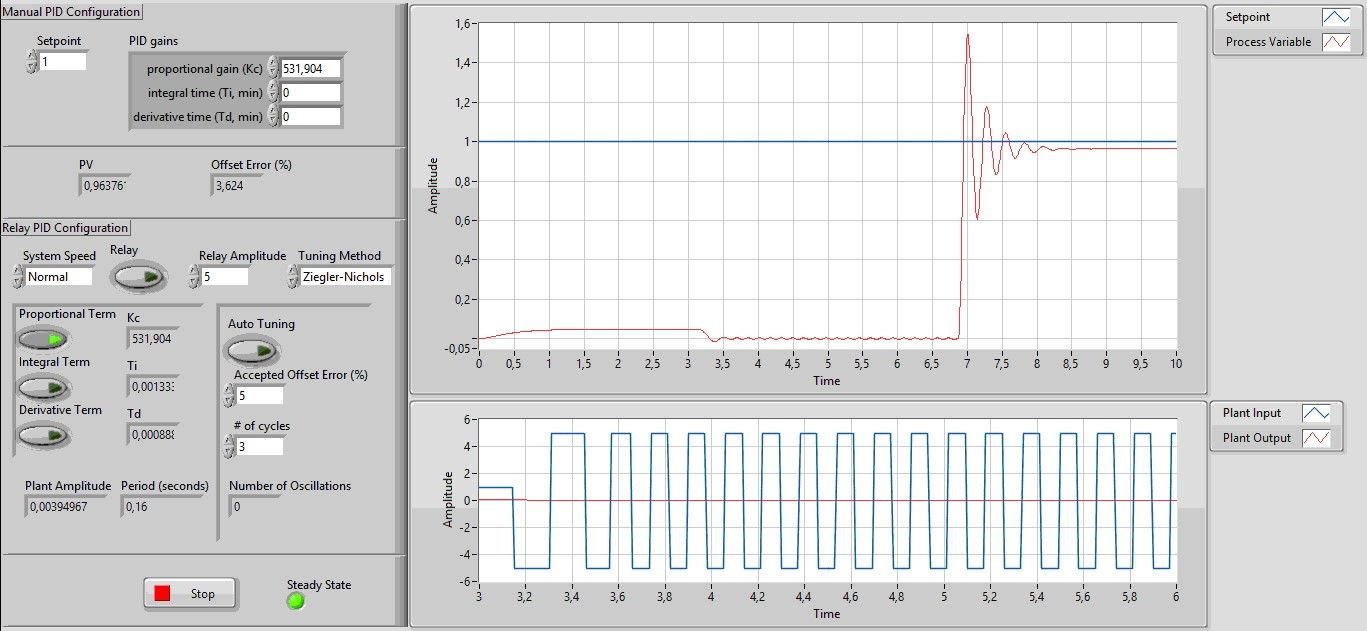
\includegraphics[width=\textwidth,height=5cm,keepaspectratio]{mass_springer_damper_proportional_control}
  \caption{Βηματική απόκριση του συστήματος Μάζα-Ελατήριο-Αποσβεστήρας με εφαρμογή αναλογικού ελέγχου}
  \label{fig:mass_springer_damper_proportional_control}
\end{figure}

\begin{figure}[h]
  \centering
  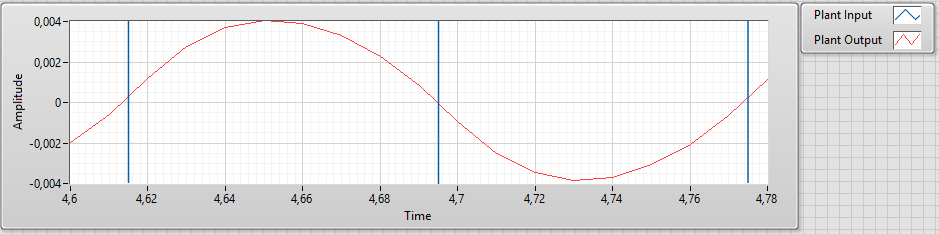
\includegraphics[width=\textwidth]{mass_springer_damper_oscillations}
  \caption{Μεγέθυνση των ταλαντώσεων του συστήματος κατά τη διάρκεια του πειράματος relay}
  \label{fig:mass_springer_damper_oscillations}
\end{figure}

\subsubsection{Αναλογικός-Ολοκληρωτικός Έλεγχος}

Το πείραμα επαναλαμβάνεται αλλά αυτή τη φορά χρησιμοποιείται και ο ολοκληρωτικός όρος προκειμένου να εξαλειφθεί το σφάλμα μόνιμης κατάστασης. Όπως φαίνεται από το Σχήμα \ref{fig:mass_springer_damper_integral_control}, η προσθήκη του ολοκληρωτικού όρου, όχι μόνο δεν μηδενίζει το σφάλμα μόνιμης κατάστασης αλλά χειροτερεύει την απόκριση του συστήματος σε σημείο να το οδηγεί να εκτελεί ταλαντώσεις γύρω από το επιθυμητό σημείο. Αυτό χωρίς αμφιβολία, είναι μία μη αποδεκτή κατάσταση.

\begin{figure}[h]
  \centering
  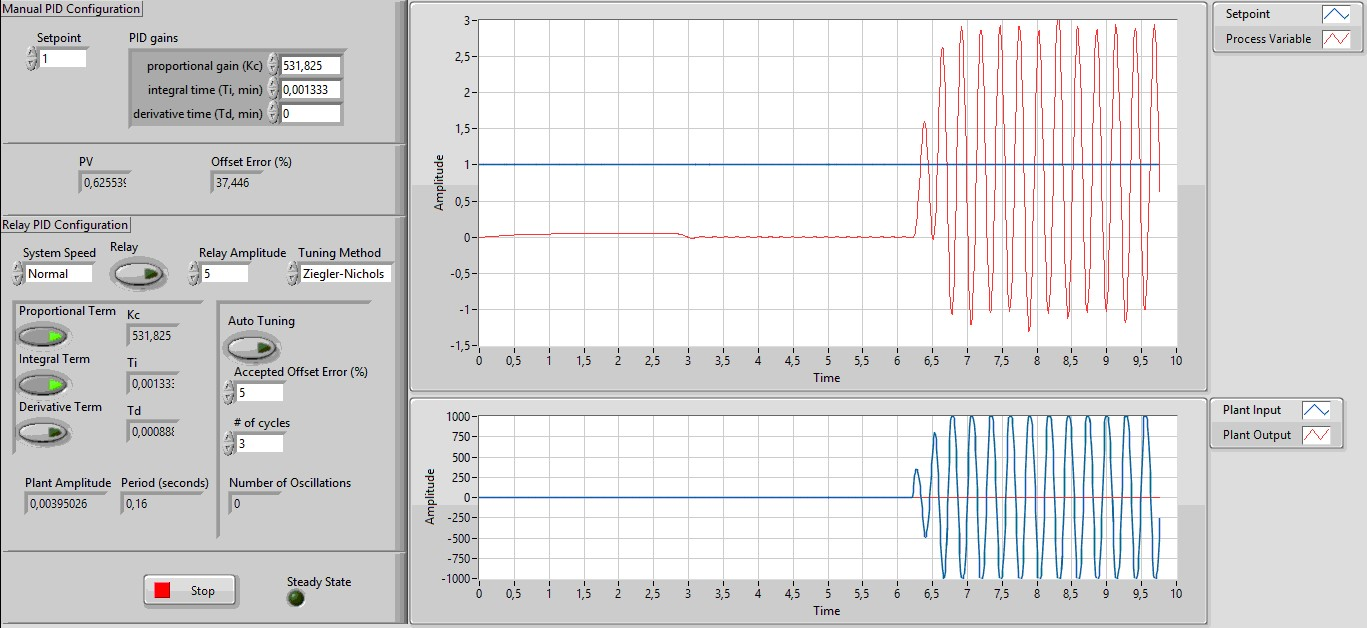
\includegraphics[width=\textwidth,height=5cm,keepaspectratio]{mass_springer_damper_integral_control}
  \caption{Βηματική απόκριση του συστήματος Μάζα-Ελατήριο-Αποσβεστήρας με εφαρμογή αναλογικού-ολοκληρωτικού ελέγχου}
  \label{fig:mass_springer_damper_integral_control}
\end{figure}

\subsubsection{Αναλογικός-Ολοκληρωτικός-Διαφορικός Έλεγχος}

Προκειμένου να βελτιωθεί η ευστάθεια του συστήματος εισάγεται και ο διαφορικός όρος. Ενώ ο ολοκληρωτικός όρος εισάγει έναν πόλο στο σύστημα, ο διαφορικός όρος εισάγει ένα μηδενικό βελτιώνοντας έτσι την ευστάθεια. Όπως φαίνεται στο Σχήμα \ref{fig:mass_springer_damper_derivative_control} η απόκριση βελτιώθηκε αισθητά. Ο έλεγχος που παρέχουν και οι τρεις όροι, όχι μόνο μηδένισε το σφάλμα μόνιμης κατάστασης όπως ήταν αναμενόμενο λόγω του ολοκληρωτικού όρου, αλλά βελτίωσε και τη μεταβατική κατάσταση του συστήματος. Η υπέρβαση, που πριν είχε ποσοστό σχεδόν $50\%$ τώρα έχει ποσοστό περίπου $20\%$. Επίσης έχει χρόνο ανύψωσης λιγότερο από ένα δευτερόλεπτο. Πλέον η απόκριση του συστήματος κρίνεται ικανοποιητική.

\begin{figure}[h]
  \centering
  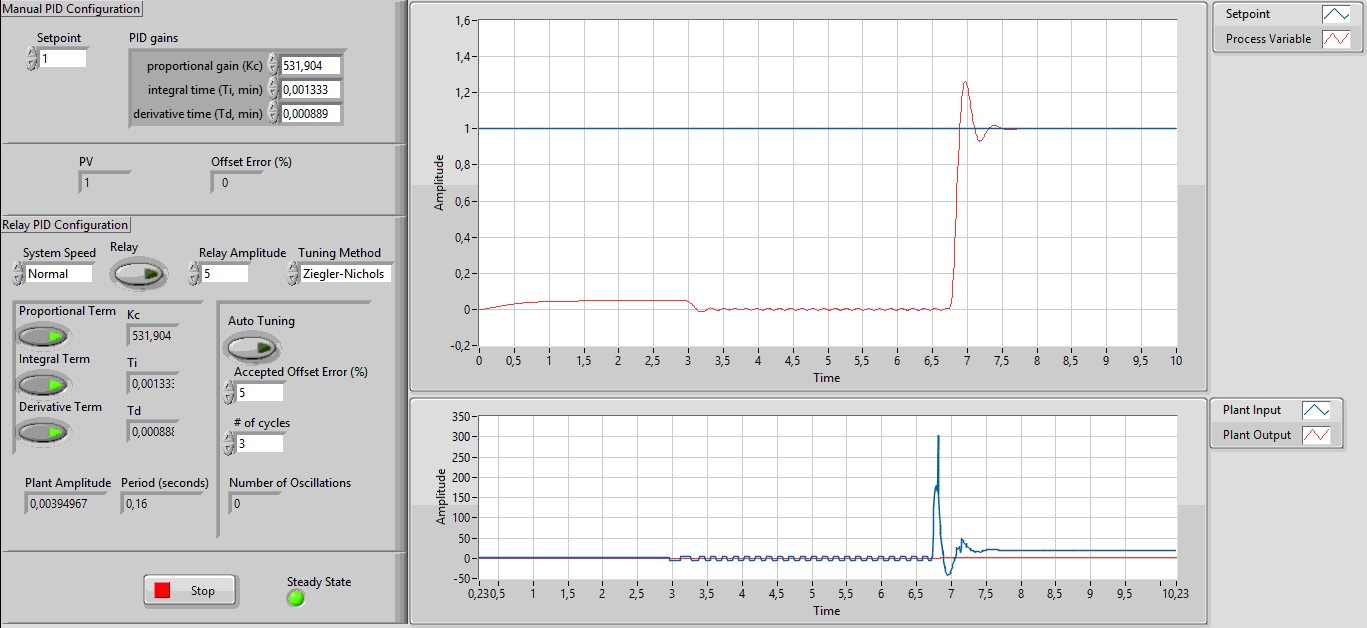
\includegraphics[width=\textwidth,height=5cm,keepaspectratio]{mass_springer_damper_derivative_control}
  \caption{Βηματική απόκριση του συστήματος Μάζα-Ελατήριο-Αποσβεστήρας με εφαρμογή αναλογικού-ολοκληρωτικού-διαφορικού ελέγχου}
  \label{fig:mass_springer_damper_derivative_control}
\end{figure}

Όπως έχει αναφερθεί κάθε διεργασία μπορεί να έχει διαφορετικές απαιτήσεις ελέγχου. Μπορεί για μία συγκεκριμένη εφαρμογή, η υπέρβαση που παρουσιάζει ο έλεγχος με αυτά τα κέρδη να μην είναι αποδεκτός. Έχει ενδιαφέρον λοιπόν να δούμε πώς ανταποκρίνεται το σύστημα σε διαφορετικές τιμές των κερδών. Ορίζοντας την επιθυμητή ταχύτητα του κλειστού συστήματος σε ``Slow" αντί για ``Normal" έχουμε την παρακάτω απόκριση. Από το διάγραμμα βλέπουμε ότι πλέον το σύστημα δεν παρουσιάζει υπέρβαση αλλά ως αντάλλαγμα αργεί αισθητά περισσότερο να φτάσει στην επιθυμητή τιμή.

\begin{figure}[h]
  \centering
  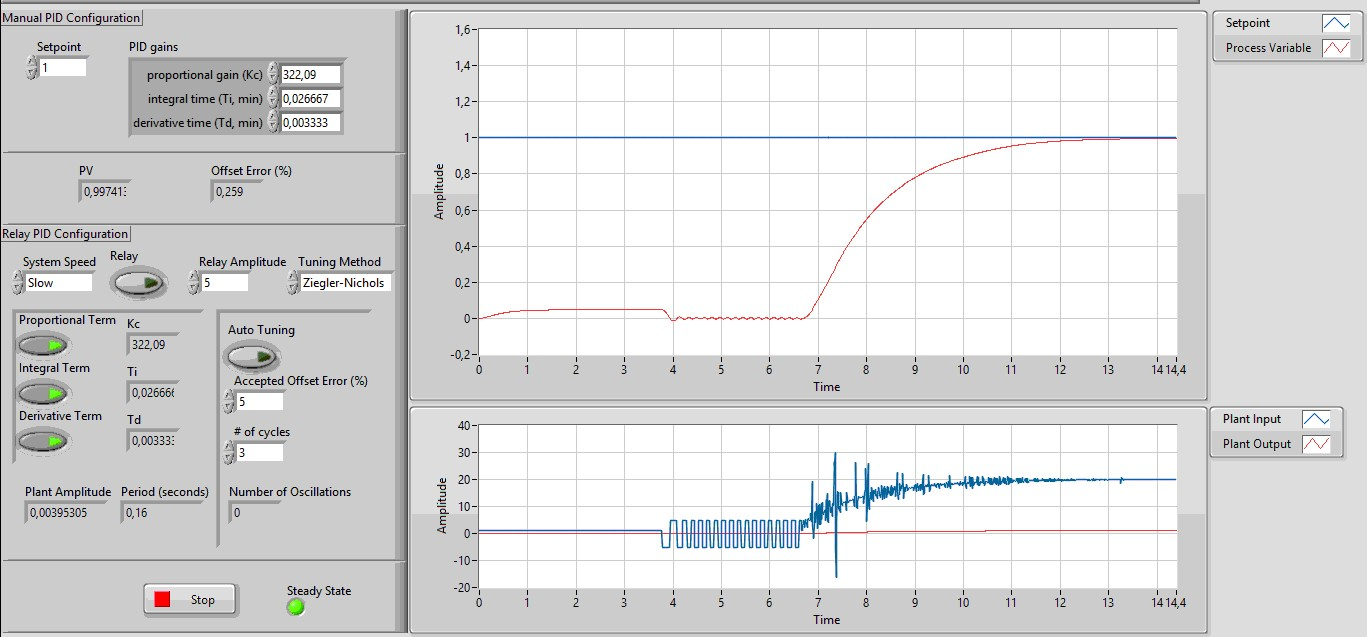
\includegraphics[width=\textwidth,height=5cm,keepaspectratio]{mass_springer_damper_ZN_slow}
  \caption{Βηματική απόκριση του συστήματος Μάζα-Ελατήριο-Αποσβεστήρας με εφαρμογή αναλογικού-ολοκληρωτικού-διαφορικού ελέγχου στη λειτουργία ``Slow"}
  \label{fig:mass_springer_damper_ZN_slow}
\end{figure}

Ακόμα, στο Σχήμα \ref{fig:mass_springer_damper_TL} φαίνεται η βηματική απόκριση του κλειστού συστήματος όταν τα κέρδη του ελεγκτή έχουν υπολογιστεί με τους τύπους Tyreus-Luyben. Η απόκριση μοιάζει σαν μια μίξη των δύο προηγούμενων αποκρίσεων. Η έξοδος του συστήματος δεν παρουσιάζει υπέρβαση, αλλά φτάνει και στην επιθυμητή τιμή μέσα σε περίπου ένα δευτερόλεπτο.

\begin{figure}[h]
  \centering
  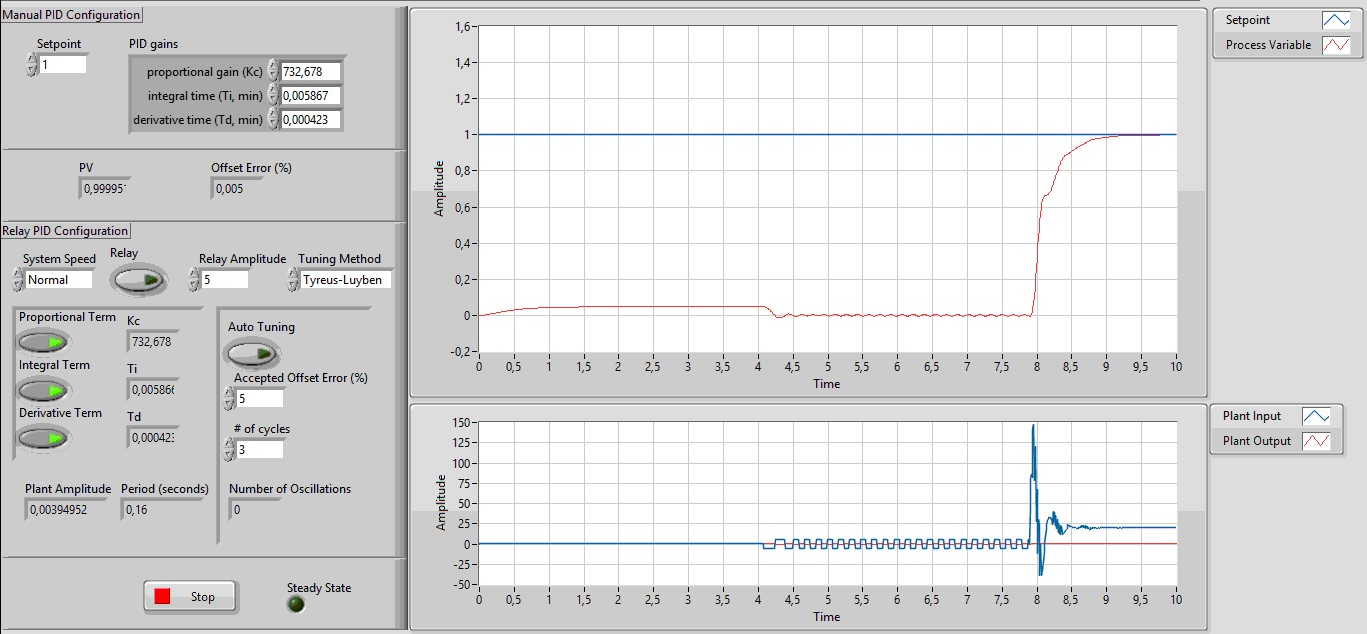
\includegraphics[width=\textwidth,height=5cm,keepaspectratio]{mass_springer_damper_TL}
  \caption{Βηματική απόκριση του συστήματος Μάζα-Ελατήριο-Αποσβεστήρας με εφαρμογή αναλογικού-ολοκληρωτικού-διαφορικού ελέγχου του οποίου τα κέρδη έχουν υπολογιστεί με τους τύπους Tyreus-Luyben}
  \label{fig:mass_springer_damper_TL}
\end{figure}



\subsubsection{Αντιμετώπιση Διαταραχών}
Στο Σχήμα \ref{fig:mass_spring_damper_disturbances} φαίνεται πώς το σύστημα αντιδράει στην ύπαρξη διαταραχών. Περίπου στο δέκατο τρίτο δευτερόλεπτο, γίνεται μια γρήγορη μεταβολή του setpoint η οποία ισοδυναμεί με μία σχεδόν στιγμιαία διαταραχή. Από το διάγραμμα της απόκρισης φαίνεται ότι το σύστημα έχει επανέλθει στην ηρεμία και έχει μηδενικό σφάλμα μόνιμης κατάστασης. 

\begin{figure}[h]
  \centering
  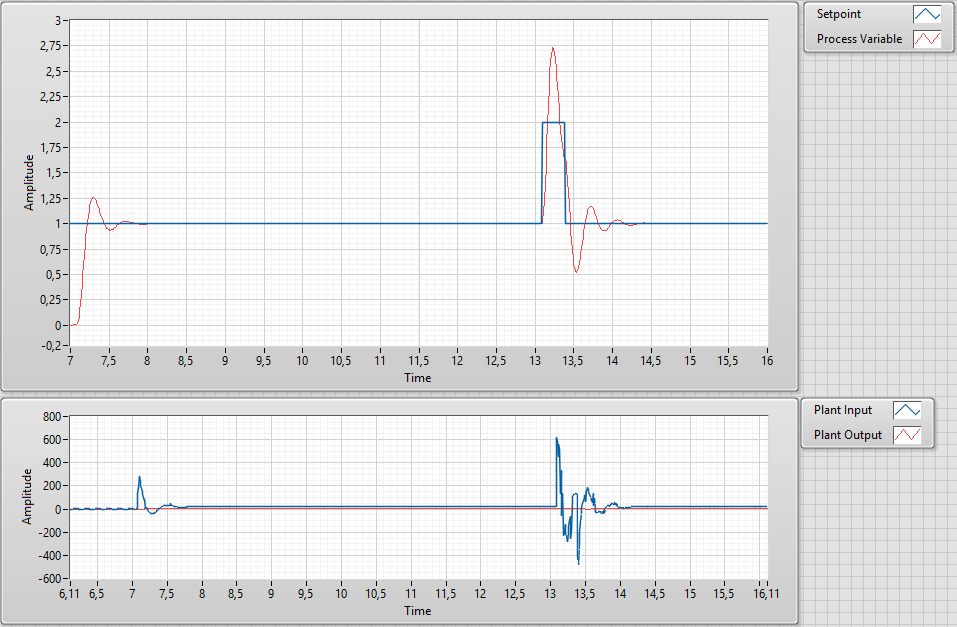
\includegraphics[width=\textwidth,height=5cm,keepaspectratio]{mass_spring_damper_disturbances}
  \caption{Αντιμετώπιση διαταραχών του αυτο-ρυθμιζόμενου PID ελεγκτή του οποίου τα κέρδη έχουν υπολογιστεί με τους τύπους Ziegler-Nichols}
  \label{fig:mass_spring_damper_disturbances}
\end{figure}

Όπως και πριν, έχει ενδιαφέρον να δούμε πώς διαχειρίζεται τις διαταραχές το σύστημα όταν τα κέρδη του ελεγκτή έχουν υπολογιστεί χρησιμοποιώντας διαφορετικούς τύπους. Έτσι, στο Σχήμα \ref{fig:mass_spring_damper_disturbances_slow} φαίνεται η προσπάθεια του ελεγκτή να ελέγξει το σύστημα σε διαταραχή, όταν τα κέρδη έχουν υπολογιστεί με τη μέθοδο Ziegler-Nichols και οι τύποι έχουν προσαρμοστεί για να δίνουν μια πιο αργή απόκριση.

\begin{figure}[h]
  \centering
  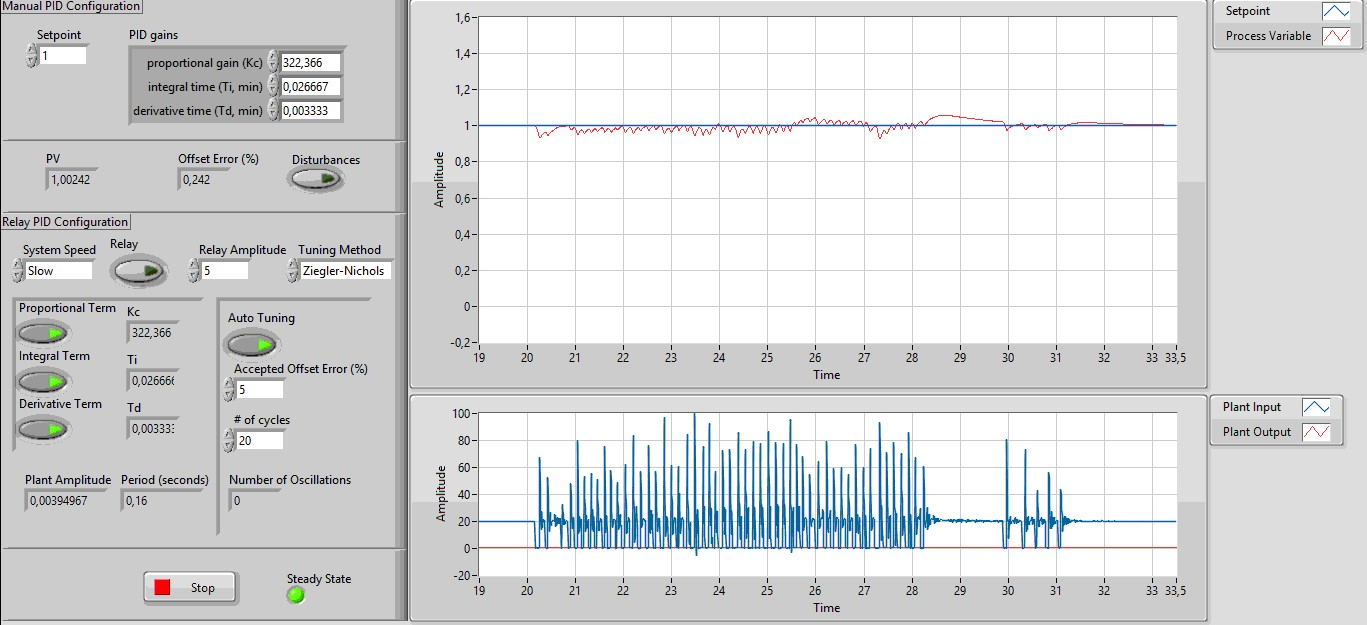
\includegraphics[width=\textwidth,height=5cm,keepaspectratio]{mass_spring_damper_disturbances_slow}
  \caption{Αντιμετώπιση διαταραχών του αυτο-ρυθμιζόμενου PID ελεγκτή του οποίου τα κέρδη έχουν υπολογιστεί με τους τύπους Ziegler-Nichols στη λειτουργία ``Slow"}
  \label{fig:mass_spring_damper_disturbances_slow}
\end{figure}

Τέλος, στο Σχήμα \ref{fig:mass_spring_damper_disturbances_TL} φαίνεται η αντιμετώπιση των διαταραχών όταν τα κέρδη έχουν υπολογιστεί με τους τύπους Tyreus-Luyben. Το σύστημα σταθεροποιείται πριν περάσει περισσότερο από ένα δευτερόλεπτο αλλά παρουσιάζει ένα μικρό ποσοστό υπέρβασης.

\begin{figure}[h]
  \centering
  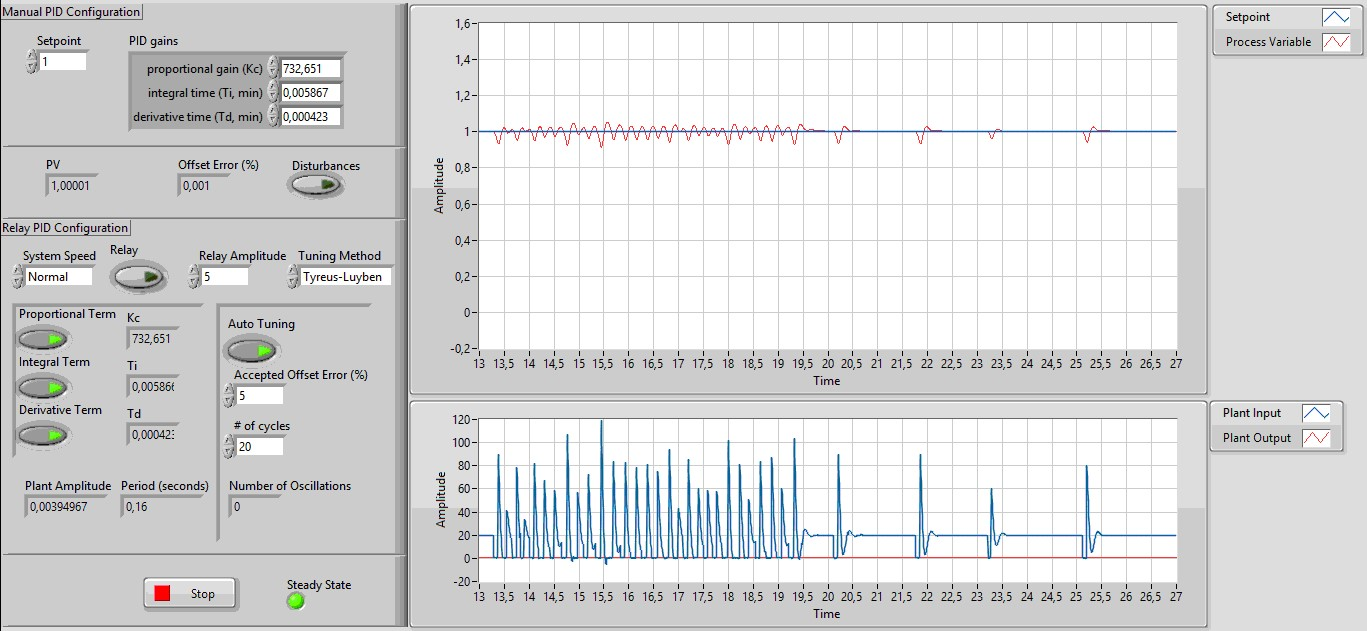
\includegraphics[width=\textwidth,height=5cm,keepaspectratio]{mass_spring_damper_disturbances_TL}
  \caption{Αντιμετώπιση διαταραχών του αυτο-ρυθμιζόμενου PID ελεγκτή του οποίου τα κέρδη έχουν υπολογιστεί με τους τύπους Tyreus-Luyben}
  \label{fig:mass_spring_damper_disturbances_TL}
\end{figure}



















